% 倍长中线 例2：D 是 BC 中点，E∈AB, EF∥AC 交 CD 延长线于 F. 证 CE=AF.
\documentclass[tikz,border=4pt]{standalone}
\usepackage{ctex}
\usepackage{amsmath}
\usetikzlibrary{calc, decorations.markings}
\begin{document}
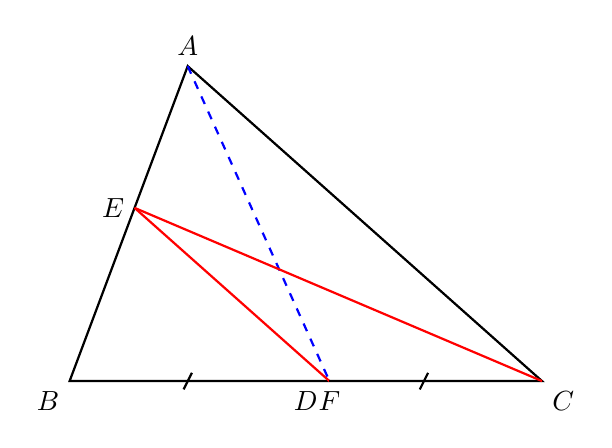
\begin{tikzpicture}[scale=1.0, thick,
  tick/.style={postaction={decorate, decoration={markings,
    mark=at position 0.5 with {\draw (-1.5pt,-3pt) -- (1.5pt,3pt);}}}}]
  \coordinate (B) at (0,0);
  \coordinate (C) at (6,0);
  \coordinate (A) at (1.5, 4);
  \coordinate (D) at (3,0);
  \coordinate (E) at ($(A)!0.45!(B)$);
  % EF ∥ AC, 过 E 作平行 AC 方向 (C-A)
  % F 在 CD 延长线上. CD 方向 = D - C = (-3,0), 延长过 D 到 D 之外
  % 求交点: 直线 EF: E + t*(C-A); 直线 CD 延长线: y=0
  % E = (A!0.45!B) = A + 0.45*(B-A) = (1.5*0.55, 4*0.55) = (0.825, 2.2)
  % C-A = (4.5, -4)
  % E.y + t*(-4) = 0 -> t = 2.2/4 = 0.55
  % F = (0.825 + 0.55*4.5, 0) = (3.3, 0)... 在 D=(3,0) 右侧
  \coordinate (F) at (3.3, 0);
  \draw (A)--(B)--(C)--cycle;
  \draw[tick] (B)--(D);
  \draw[tick] (D)--(C);
  \draw[red] (E)--(F);
  \draw (C)--(F);
  \draw[blue, dashed] (A)--(F);
  \draw[red] (C)--(E);
  \node[above] at (A) {$A$};
  \node[below left] at (B) {$B$};
  \node[below right] at (C) {$C$};
  \node[below] at (D) {$D$};
  \node[left] at (E) {$E$};
  \node[below] at (F) {$F$};
\end{tikzpicture}
\end{document}
